The following three types of image filters have been designed:
\begin{itemize}
\item Red-Filter
\item Green-Filter
\item Blue-Filter
\end{itemize}
These simple filters generates data, that just includes the red/green/blue values of a 32-Bit RGB data set, regarding to the chosen logic of the dynamic partial reconfiguration application. Figure \ref{fig:imagefilter} describes the principle of the filter functionality. The logic of these filters is connected to the AXI-Lite Bus with the same Wrapper-Interface and is addressable by a common Linux-Device-Driver.
\begin{figure}[h]
\centering
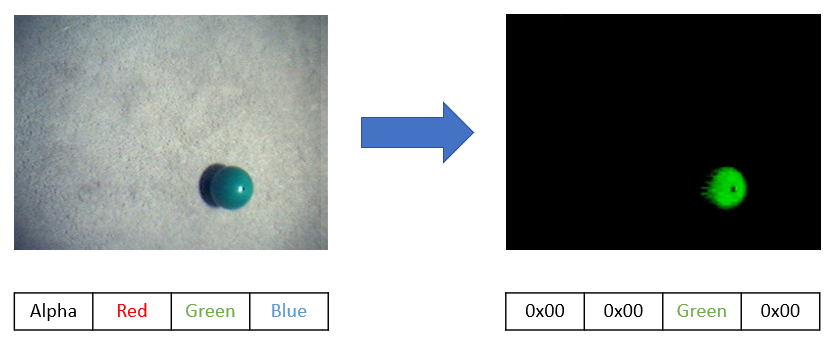
\includegraphics[width=1\textwidth]{sections/methodology/ImageFilter.PNG}
\caption{\label{fig:imagefilter} Green Filter example}
\end{figure}